% !TEX TS-program = luatex
% Ahmed Elshaabany's Pro. CV LaTeX Template
%
% Author:
% Ahmed Elshaabany
%
% Template license:
% CC BY-SA 4.0 (https://creativecommons.org/licenses/by-sa/4.0/)

\documentclass[localFont,alternative]{documentMETADATA}
\name{Ahmed}{Elshaabany}
\tagline{Mobile / Frontend engineer | Scrum Master}
% \begin{wrapfigure}{r}{0.25\textwidth}
%     \centering
%     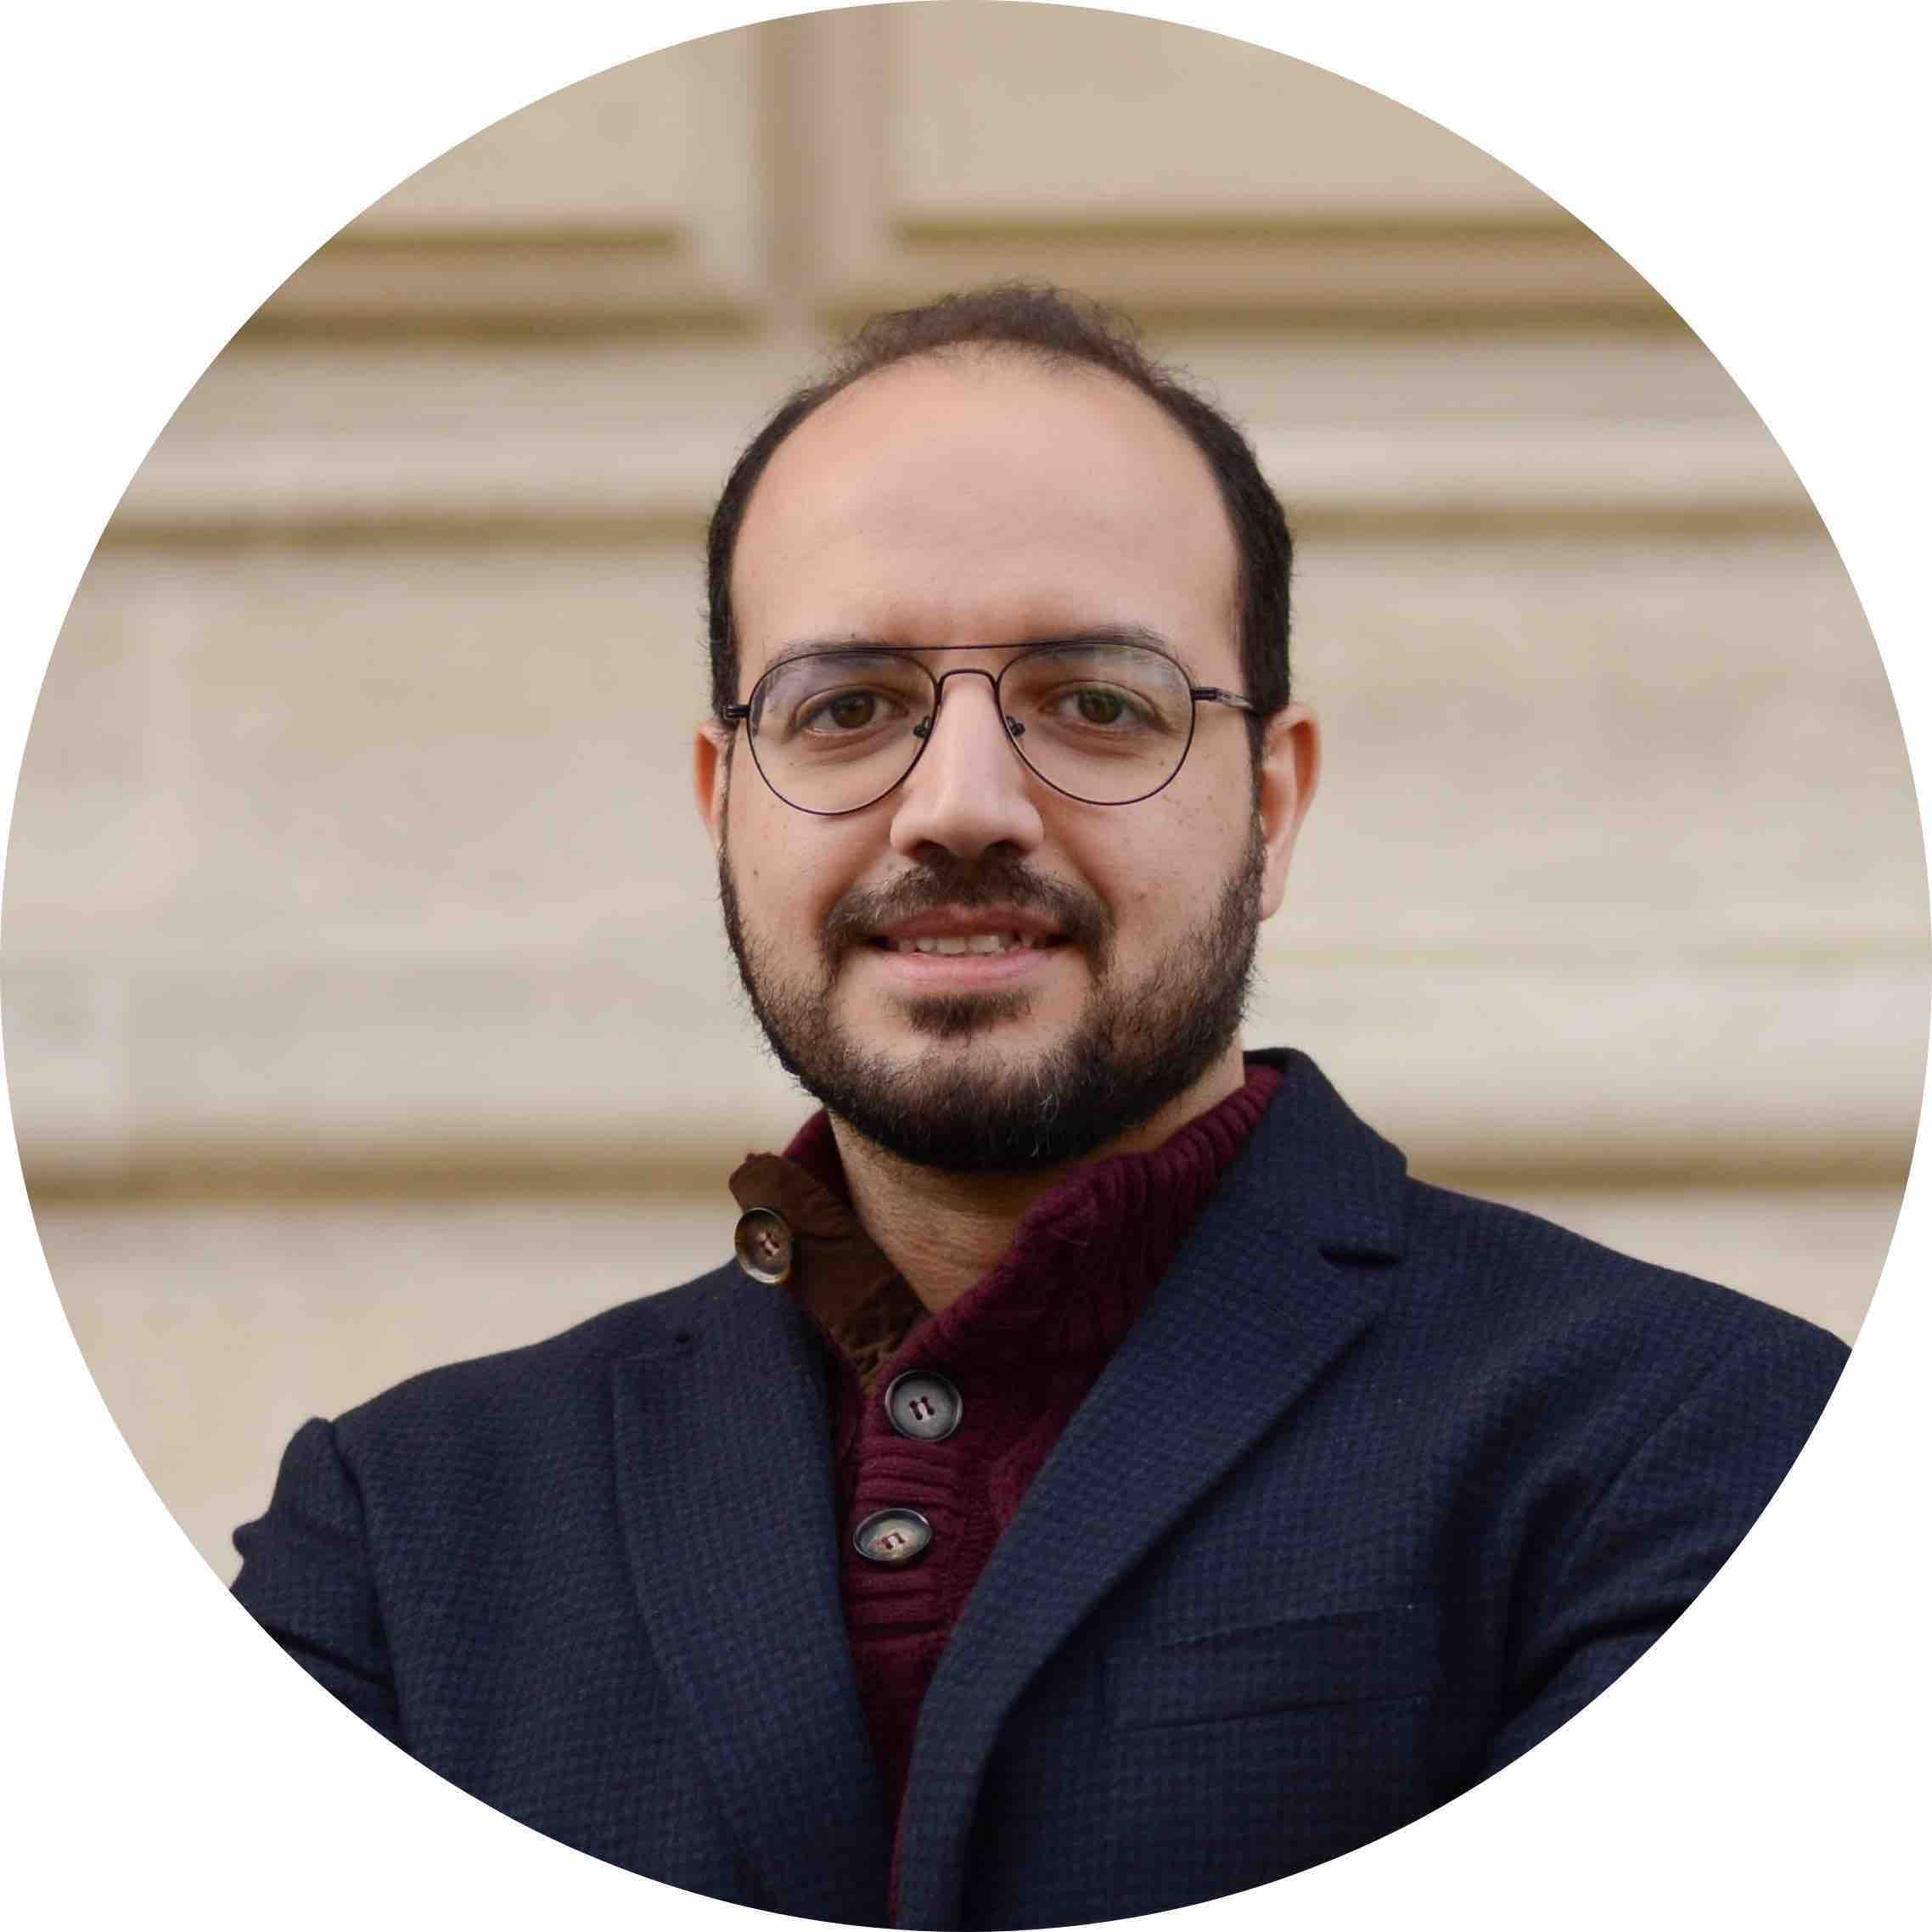
\includegraphics[width=0.25\textwidth]{me-circle-2}
% \end{wrapfigure}
% \vspace{1.2cm}
\photo{1.5cm}{me-circle-2}
\socialinfo{
    \begin{tabular}{l|l}
        \address{Frankfurt am Main, Germany}    & \smartphone{+49 1525 8141 595}     \\
    	\email{ahmed.elshabany@gmail.com}       & \linkedin{aelshaabany}             \\
    	\github{zaprogrammer}                   & \gplay{zaprogrammer}               \\
    % 	\personalLink{personal-email}\\
    % 	\infos{U.S. Citizen}
    \end{tabular}
}

\begin{document}

	\makecvheader

	\makecvfooter
		{\textsc{}} %\selectlanguage{english}\today
		{\textsc{Ahmed Elshaabany - CV}}
		{\thepage}

	% YAAC Another Awesome CV LaTeX Template
%
% This template has been downloaded from:
% https://github.com/darwiin/yaac-another-awesome-cv
%
% Author:
% Christophe Roger
%
% Template license:
% CC BY-SA 4.0 (https://creativecommons.org/licenses/by-sa/4.0/)
\par{
Goal-oriented professional with 13+ years of experience and a proven knowledge of software development, 6 years in Android, cross-platform mobile apps, and websites. Successfully delivering various products for many companies, aiming to leverage my skills to successfully fill the Mobile/Frontend engineer role at your company.
}                % Research Statement
	% YAAC Another Awesome CV LaTeX Template
%
% This template has been downloaded from:
% https://github.com/darwiin/yaac-another-awesome-cv
%
% Author:
% Christophe Roger
%
% Template license:
% CC BY-SA 4.0 (https://creativecommons.org/licenses/by-sa/4.0/)
%Section: Work Experience at the top
\vspace{0.1cm}
\sectionTitle{Professional Experience}{\faSuitcase}
%\renewcommand{\labelitemi}{$\bullet$}
\begin{experiences}
    \experience
        {savedroid AG (Fintech)}   {Mobile/Frontend engineer, Scrum Master}
        {Frankfurt, Germany}
        {Oct 2019}{Present}
        {
            \begin{itemize}
                \item Develop company's android app savedroid and migrate java code to kotlin.                        
                \item Developing mobile applications using React native utilising AWS services.                    
                \item Handle product CD processes through different channels like
                Bitrise and releases to store.                
                \item Manage scrum events (daily huddles, Retros, Sprint reviews,...).                                                                    
            \end{itemize}
        }
        {Android, Java, Kotlin, Reactnative, Typescript, Firebase, AWS, Bitrise, Mixpanel, JIRA, Bitbucket}
    \emptySeparator
    \experience
        {AHBS (Healthcare)}   {Mobile/Web Technical Lead, Scrum Master}
        {Alexandria, Egypt}
        {Jun 2018}{Jul 2019}
            {
                \begin{itemize}
                    \item Led 11 engineers in both teams of Mobile (Android/iOS)
                    and Websites through developing company’s products.                           
                    \item Raised team performance by more than 50\% through processes
                    and tools, like CD, \\Automation testing, Scrum and Kanban.
                    \item Raised company products’ KPIs in performance and quality.  
                    \item Coach the teams through the agile process.                
                    \item Shaped early stage of company's PHR product.
                \end{itemize}
            }
            {Android, Java, Wordpress, HTML, CSS, Javascript, TFS, Scrum/Kanban}
    \emptySeparator
    \experience
        {Macber-eg (Startup)}   {Technical Development Lead}
        {Cairo, Egypt}
        {Dec 2017}{May 2018}
            {
                \begin{itemize}
                    \item Develop mobile applications using Ionic framework for both
                    Android and iOS
                    \begin{itemize}
                        \item Levari Client/Agent: 2 Chatting applications for Levari
                        company Clients and Agents using \\Socket.IO                
                        \item  Jametna: Booking application for houses and special
                        occasions in KSA. 
                    \end{itemize}
                    \item Develop company's Registration System using NodeJS and Electron.                          
                    \item Manage company’s software projects.                                                      
                    \item Technical leading the team through the SDLC.
                \end{itemize}
            }
            {Ionic 2, Cordova, Angular, Typescript, Javascript, NodeJS, Electron,
            SocketIO, Git}
    \emptySeparator
    \experience
        {Bondinco (Infotainment)}   {Front-end consultant (Mobile / Web)}
        {Dubai, UAE}
        {Jul 2017}{Oct 2017}
        {
        %   (\href{https://www.edqm.eu/fr/eTACT-1466.html}{\textbf{\em accident}}).
            \begin{itemize}
                \item Rebuilt the company’s product Lollibond using latest technology
                stacks.                               
                \item Successfully delivered the product in 3 months after being stuck in development for 1.5 years.            
                \item Modernized development frameworks and tools.
                \item Initiate architecture for company’s mobile app product.
                \item Trained other developers on updated technologies and tools like Angular5, Git, ...
            \end{itemize}
        }
        {Angular 2/5, Javascript, CSS, HTML, Git, Sass, Material}
    \emptySeparator
    \experience
        {CIT Global (FinTech)}   {Technical Team Leader}
        {Cairo, Egypt}
        {Jan 2014}{ Jun 2017}
        {
            \begin{itemize}
                \item Lead the frontend development team of the company’s breakthrough
                mobile payment solution Vericash.                                            
                \item Communicate with and report to the project manager about system
                new requirements, tasks schedules, and team performance.
                \item Develop new features and fix issues in the frontend applications.
                \item Help in updating and migrating the current used technologies to up-to-date ones and conduct training to colleagues about those
                technologies.
                \item Train the team on new technologies.
                \item Applications deployment and delivery to customers.
            \end{itemize}
        }
        {Android, Java, Cordova, Angular, Onsen UI, mobile security}  
    \emptySeparator
    \experience
        {Zerowire Labs (Startup)}   {Mobile team lead}
        {Cairo, Egypt}
        {Dec 2012}{Oct 2013}
        {
            \begin{itemize}
                \item Lead a team of talented mobile developers to craft applications for various mobile platforms (iOS / Android / Blackberry) using Agile, Scrum methodology to ensure delivery of high quality work with every monthly iteration.                                            
                \item Gather input from project leads and customers for employee 
                performance reviews and document information.
                \item Creating wireframes, storyboards, user flows, process flows for new projects.
                \item Manage the hiring procedure of new development employees.
                \item Directly communicate with clients for requirement gathering and technical issues solving.
            \end{itemize}
        }
        {Blackberry, Android, Java, Agilefant}
    \emptySeparator
    \experience
        {Zerowire Labs (Startup)}   {Senior Software Engineer}
        {Cairo, Egypt}
        {Aug 2011}{Nov 2012}
        {
            \begin{itemize}
                \item Develop mobile applications for blackberry.
            \end{itemize}
        }
        {Blackberry, Java, J2me, Agile}
    \emptySeparator
    \experience
        {iKD (Startup)}   {Web Applications Developer}
        {Cairo, Egypt}
        {Jan 2011}{May 2011}
        {
            \begin{itemize}
                \item Contribute in developing DMS and CMS products.
                \item Developing websites for other companies such as ForeSight.com.
                \item Migrating the company’s products to mobile-based applications as
                well as developing mobile applications upon request.
            \end{itemize}
        }
        {ASP.NET, {C\#}, MVC, Telerik, HTML, CSS, Javascript}
    \emptySeparator
    \experience
        {SDG}   {Systems Engineer}
        {Dubai, UAE}
        {Sep 2008}{Nov 2010}
        {
            \begin{itemize}
                \item Developed and implemented a web-based system (e-Transport)
                on-site for the RTA authority in Dubai, to manage the different modules in the Public Transport Agency (PTA) like accidents, KPIs, Drivers training, Tasks management, etc.
                \item Developed web-based applications and websites that transform the existing manual systems to automated digitised systems.
                \item Communicating with customers periodically to get their feedback about the system and insure their satisfaction.
                \item Installed and configured systems such as infrastructure
                applications or Asset Management applications.
                \item Develop and maintain installation and configuration procedures.
            \end{itemize}
        }
        {ASP.NET, {C\#}, MVC, Telerik, HTML, CSS, Javascript}
    \emptySeparator
    \experience
        {Education (Training)}   {Systems Engineer}
        {Cairo, Egypt}
        {Feb 2009}{Sep 2009}
        {
            \begin{itemize}
                \item Develop an internal web-based application for the company. The application modules included such as HR, Training, Testing, Customer
                Service. The system was developed using Java, JSP/Servlets, DB2
                database and Websphere application server (WAS).
                \item Develop and implement the website for the company. The website was developed using Java, JSP/Servlets, DB2 database and Websphere application server (WAS).
                \item Providing training for IBM courses such as Websphere application
                server (WAS), Java, DB2.
            \end{itemize}
        }
        {Java, J2EE, JSP, Servlets, Java beans, WAS, DB2, HTML, CSS, IBM Portal}
    \emptySeparator
    \experience
        {IBM}   {Web development Scholarship}
        {Cairo, Egypt}
        {Feb 2008}{Jan 2009}
        {
                    
            \begin{itemize}
                \item IBM Web Application Development Diploma.
            \end{itemize}
        }
        {Java, J2EE, JSP, Servlets, Java beans, IBM WAS, IBM RAD, IBM DB2, HTML, CSS, IBM WebSphere Portal, XML}
    \emptySeparator
    \experience
        {e3050 (eCommerce)}   {Web Developer}
        {Cairo, Egypt}
        {Sep 2007}{Jan 2008}
        {
            \begin{itemize}
                \item Developed and maintained an internal web-based e-Commerce 
                application to handle the different operations in the transactions for the company from buying and selling, using C\#, ASP.NET and SQL Server 
                database.
                \item Work as an Administrator for Windows Server 2003.
                \item Research and recommend innovative, and where possible automated approaches for system administration tasks.
                \item Perform daily system monitoring, verifying the integrity and availability of all hardware, server resources, systems and key processes, reviewing system and application logs, and verifying completion of 
                scheduled jobs such as backups.
                \item Perform regular security monitoring to identify any possible intrusions.
            \end{itemize}
        }
        {ASP.NET, {C\#}, SQL Server, HTML, CSS, Javascript, Windows server} 
\end{experiences}
	        	% Section Professional Experience
	% YAAC Another Awesome CV LaTeX Template
%
% This template has been downloaded from:
% https://github.com/darwiin/yaac-another-awesome-cv
%
% Author:
% Christophe Roger
%
% Template license:
% CC BY-SA 4.0 (https://creativecommons.org/licenses/by-sa/4.0/)

%Section: Qualifications -> Education
\sectionTitle{QUALIFICATIONS}{\faGraduationCap}

% \begin{scholarship}
% 	\scholarshipentry{Institute of Computer Information Technology in Avionics and Aerospace}
% 					{B. Sc. in Computer and Information Technology}
% 	\scholarshipentry{Arab Academy for Science, Technology and Maritime Transport}
% 					{Higher Diploma in Information Technology}
% % 	\scholarshipentry{2004}
% % 					{BTS Informatique de Gestion option administrateurs de réseaux}
% % 	\scholarshipentry{2000}
% % 					{Baccalauréat Scientifique option Mathématiques}
% \end{scholarship}

\begin{experiences}
    \experience
    {}   {Higher Diploma in Information Technology}{Egypt}{2011}
    {2012} {
            \begin{itemize}
                \item \textbf{Arab Academy for Science, Technology and Maritime Transport}
            \end{itemize}
        }{}
    \emptySeparator
    \experience
    {}   {B. Sc. in Computer and Information Technology}{Egypt}{2003}
    {2007} {
            \begin{itemize}
                \item \textbf{Institute of Computer Information Technology in Avionics and Aerospace}
            \end{itemize}
        }{}
\end{experiences}			% Section Qualifications & Education
%   % YAAC Another Awesome CV LaTeX Template
%
% This template has been downloaded from:
% https://github.com/darwiin/yaac-another-awesome-cv
%
% Author:
% Christophe Roger
%
% Template license:
% CC BY-SA 4.0 (https://creativecommons.org/licenses/by-sa/4.0/)

%Section: Scholarships and additional info
\sectionTitle{Publications}{\faBook}

\begin{scholarship}
	\scholarshipentry{2007}
					{Master STIC Professionel filière MBDS de l'Université de Nice Sophia Antipolis (Master Informatique spécialité Multimédia, Base de Données et intégration de Systèmes)}
	\scholarshipentry{2005}
					{Licence Sciences et Technologies, Mention Informatique, de l'Université de Nouvelle-Calédonie}
	\scholarshipentry{2004}
					{BTS Informatique de Gestion option administrateurs de réseaux}
	\scholarshipentry{2000}
					{Baccalauréat Scientifique option Mathématiques}
\end{scholarship}        % Section Publications, presentations,...
	% YAAC Another Awesome CV LaTeX Template
%
% This template has been downloaded from:
% https://github.com/darwiin/yaac-another-awesome-cv
%
% Author:
% Christophe Roger
%
% Template license:
% CC BY-SA 4.0 (https://creativecommons.org/licenses/by-sa/4.0/)

%Section compétences
\sectionTitle{Technical Skills}{\faTasks}

\begin{keywords}
		\keywordsentry{Mobile}{\textbf{Android} (\textbf{Java}, \textbf{Kotlin}), Flutter, React native, Ionic (1,2/3), Cordova (Phonegap), Mobile Security}
		
		\keywordsentry{Web}{Angular (1,2/5), HTML5, CSS3, ES6, XML, REST/SOAP Web-Services APIs, XMPP, Socket, PHP, NodeJS, Gulp, Webpack.}
		
		\keywordsentry{Testing}{ JUnit test, FindBugs, SonarCube, TestIO}
		
		\keywordsentry{CI/CD}{Octopus, Jenkins, Gitlab, Fastlane, Bitrise}
		
		\keywordsentry{DBs}{ORMs, Sqlite, MySQL, MS SQL Server}
		
		\keywordsentry{IDEs and Tools}{Android Studio, IntelliJ, XCode, Adobe PhotoShop, Docker, SourceTree, Sympli, (X)AMP Stacks}
		
		\keywordsentry{Project Management}{TFS, Jira, Trello, MS Project, Agile(Scrum, Kanban)}
		
		\keywordsentry{Platforms}{Mac OSX, MS (Administrator), Linux (Power User)}
\end{keywords}				    % Section Skills
% 	\input{section_interets}				% Section interests
	% Awesome Source CV LaTeX Template
%
% This template has been downloaded from:
% https://github.com/darwiin/awesome-neue-latex-cv
%
% Author:
% Christophe Roger
%
% Template license:
% CC BY-SA 4.0 (https://creativecommons.org/licenses/by-sa/4.0/)

%Section: Project
\sectionTitle{Projects}{\faLaptopCode}

\begin{projects}
% 	\project
% 	{Simply City}{2017 - 2018}
%  	{\website{https://www.simplycity.nc}{https://www.simplycity.nc} \website{https://innovation.engie.com/fr/news/actus/territoires/simply-city-lappli-qui-simplifie-la-ville-au-ces-2018-avec-engie/8156}{Présentation CES 2018} }
% 	{Simply City est une application mobile, gratuite et participative destinée à tous les habitants, visiteurs et touristes qui séjournent dans une ville. L’application permet de connaître toutes les informations et services utiles en temps réel.}
% 	{Ionic 3,Typescript,Javascript,Visual Studio Code}
				
% 	\project
% 	{YAAC Another Awesome CV}{2013 - 2018}
% 	{\github{darwiin/yaac-another-awesome-cv} \website{https://www.overleaf.com/latex/templates/awesome-source-cv/wrdjtkkytqcw}{Template sur Overleaf}}
% 	{Template \LaTeX pour Curiculum Vitæ utilisant les icônes \href{https://fontawesome.com}{Font Awesome} et la police de caractère \href{https://fonts.google.com/specimen/Source+Sans+Pro}{Adobe Source Sans Pro}. YAAC Another Awesome CV a d'abord été créé comme un template simple pour CV à vocation technologique.}
% 	{\LaTeX,Sublime Text}
\end{projects}                % Section Projects
% 	% YAAC Another Awesome CV LaTeX Template
%
% This template has been downloaded from:
% https://github.com/darwiin/yaac-another-awesome-cv
%
% Author:
% Christophe Roger
%
% Template license:
% CC BY-SA 4.0 (https://creativecommons.org/licenses/by-sa/4.0/)

%Section: Scholarships and additional info
\sectionTitle{Outreach and Volunteering}{\faGraduationCap}

\begin{scholarship}
	\scholarshipentry{2007}
					{Master STIC Professionel filière MBDS de l'Université de Nice Sophia Antipolis (Master Informatique spécialité Multimédia, Base de Données et intégration de Systèmes)}
	\scholarshipentry{2005}
					{Licence Sciences et Technologies, Mention Informatique, de l'Université de Nouvelle-Calédonie}
	\scholarshipentry{2004}
					{BTS Informatique de Gestion option administrateurs de réseaux}
	\scholarshipentry{2000}
					{Baccalauréat Scientifique option Mathématiques}
\end{scholarship}   % Section Professional Outreach and volunteering
% 	% YAAC Another Awesome CV LaTeX Template
%
% This template has been downloaded from:
% https://github.com/darwiin/yaac-another-awesome-cv
%
% Author:
% Christophe Roger
%
% Template license:
% CC BY-SA 4.0 (https://creativecommons.org/licenses/by-sa/4.0/)

%Section: Scholarships and additional info
\sectionTitle{Teaching and Mentoring}{\faGraduationCap}

\begin{experiences}
  \experience
    {Aujourd'hui}   {Architecte logiciel | Développeur/Concepteur Senior JEE}{EPI}{Nouvelle-Calédonie}
    {Décembre 2015} {
                      \begin{itemize}
                        \item Reconstruction de la plateforme d'intégration                        
                        \item Migration de l'ensemble des projets Java sous Maven                    
                        \item Evolutions et corrections des bugs du framework de développement interne                
                        \item Veille technologique                                                                    
                      \end{itemize}
                    }
                    {Apache Tomcat, IntelliJ Idea, Eclipse, Maven, Spring Boot, Jenkins, Nexus}
  \emptySeparator
\end{experiences}      % Section Teaching and Mentoring
	% YAAC Another Awesome CV LaTeX Template
%
% This template has been downloaded from:
% https://github.com/darwiin/yaac-another-awesome-cv
%
% Author:
% Christophe Roger
%
% Template license:
% CC BY-SA 4.0 (https://creativecommons.org/licenses/by-sa/4.0/)

%Section: Scholarships and additional info
\sectionTitle{Certifications}{\faAward}

\begin{scholarship}
	\scholarshipentry{2008} {IBM Certified DB2 Associate (IBM, Egypt)}
	\scholarshipentry{2008} {IBM Certified Associate Developer (IBM, Egypt)}
	\scholarshipentry{2008} {IBM Certified Application Developer (IBM, Egypt)}
	\scholarshipentry{2008} {IBM Certified System Administrator (IBM, Egypt)}
\end{scholarship}          % Section Certifications
	% YAAC Another Awesome CV LaTeX Template
%
% This template has been downloaded from:
% https://github.com/darwiin/yaac-another-awesome-cv
%
% Author:
% Christophe Roger
%
% Template license:
% CC BY-SA 4.0 (https://creativecommons.org/licenses/by-sa/4.0/)

%Section: Languages
\twocolumnsection
{\sectionTitle{Languages}{\faComments}
\begin{skills}
	\skill{English}{4}
	\skill{Arabic}{5}
	\skill{German}{1}
\end{skills}}
{\sectionTitle{Forces}{\faPlus}
\vspace{1em}
\begin{itemize}
	\item Passioné
	\item Motivé                    
    \item Autonome
\end{itemize}
}
				% Section languages, Forcses
	% YAAC Another Awesome CV LaTeX Template
%
% This template has been downloaded from:
% https://github.com/darwiin/yaac-another-awesome-cv
%
% Author:
% Christophe Roger
%
% Template license:
% CC BY-SA 4.0 (https://creativecommons.org/licenses/by-sa/4.0/)

%Section: Références
\sectionTitle{References}{\faQuoteLeft}

\begin{referees}
	\referee
		{Jon Snow}
		{Lord Commander}
		{Night's Watch}
		{john.snow@nightwatch.org}
		{+687 987 654}
	\referee
		{Eddard Stark}
		{King of the North}
		{Winterfell}
		{e.stark@winterfell.org}
		{+33 1 23 45 67 90}
\end{referees} 				% Section references
	
\end{document}